\subsection{Content Management System}
\index{CMS}
Unternehmen verwenden Webpräsenzen, um sich online zu präsentieren. Dabei liegt der Fokus des Managements darauf, Informationen schnell und aktuell dem Kunden zur Verfügung zu stellen. Um dies zu erreichen, werden \acf{cms} verwendet. Diese erleichtern die Trennung von Inhalt (z. B. Texte, Bilder, Videos etc.), Layout und Struktur \cite[S.1 ff.]{spo09}. Somit muss sich ein Redakteur nicht mit dem Aussehen der Webpräsenz beschäftigen und kann sich nur auf den Inhalt fokussieren. \\
Ein \ac{cms} bietet zumeist eine Vielzahl an Funktionalitäten. Dazu gehören das Erstellen und Strukturieren von Inhalten, eine Mehrbenutzerfähigkeit und administrative Funktionen zum Verwalten besagter Nutzer \cite[S. 55]{spo09}.  Die Verwendung erfolgt über eine grafische Bedienoberfläche, um den Umgang mit dem System auch technisch weniger affinen Menschen zu vereinfachen. Diese ist generell über einen Webbrowser aufzurufen und zu verwenden. Somit benötigt ein Autor keine Zusatzsoftware und kann ortsungebunden arbeiten \cite[S. 19 f.]{bon11}. \\
Genau genommen handelt es sich um ein \ac{cms} für die Verwaltung von Webpräsenzen um ein \ac{wcms}. Der Begriff \ac{cms} wird aber häufig mit dem Begriff \ac{wcms} gleichgesetzt.

\subsubsection{Adobe Experience Manager}
\label{sec:aem}\index{AEM}
\acf{aem} ist ein ursprünglich von Day Software und dem Namen CQ entwickeltes \ac{cms}, das im Jahr 2010 von Adobe aufgekauft und nun unter neuem Namen von selbigem weiterentwickelt wird. Dieses ist in der Programmiersprache Java entwickelt, welche sich durch ihre Plattformunabhängigkeit auszeichnet. \ac{aem} gehört zu der \ac{amc} und ist mit den anderen darin enthaltenen Produkten kompatibel. Zu diesen gehören unter anderem Werkzeuge für die Analyse, das Erstellen von Zielgruppenprofilen und die Optimierung von Medieninhalten \cite[S. 1-2]{Incorporated2015}. \\
Adobe empfiehlt generell die Verwendung von drei laufenden Instanzen, jeweils auf voneinander unabhängigen Servern. Zunächst wäre hier die \quotes{Author}-Instanz zu nennen. In dieser können Autoren Inhalte erstellen, bearbeiten und administrieren. Sobald diese bereit für die Besucher sind, werden sie an die \quotes{Publisher}-Instanz weitergegeben und veröffentlicht. Um die Performance zu verbessern, empfiehlt es sich, noch eine \quotes{Dispatcher}-Instanz zu verwenden. Diese läuft auf einem Webserver und speichert die vom Publisher generierten Webseiten zwischen. Vom Benutzer generierte Inhalte, wie zum Beispiel Kommentare, werden vom Dispatcher entgegengenommen und an den Publisher weitergeleitet \cite[S. 1-3 f.]{Incorporated2015}.

\paragraph{JCR}
\ac{aem} verwendet das \ac{api} des \ac{jcr}. Diese \ac{api} wird in der aktuellen Version 2.0 vom Java Community Process spezifiziert und unter der Bezeichnung JSR-283 veröffentlicht. Sie dient dazu, über standardisierte Schnittstellen auf Inhalte zuzugreifen. Der Austausch von Inhalten zwischen einzelnen Implementierungen von \ac{jcr} ist somit möglich. \\
Bei \ac{jcr} sind Inhalte in Form von Knoten und Eigenschaften abgelegt. An der Spitze gibt es einen Wurzelknoten und jeder Knoten kann beliebig viele Kindknoten besitzen, womit eine Baumstruktur entsteht. Zudem kann jeder Knoten eine beliebige Anzahl an Eigenschaften besitzen, welche aus Name-Wert-Paaren bestehen. Jede Eigenschaft erhält einen Typ, der angibt, was für den Wert eingetragen werden darf, beispielsweise eine Zeichenkette (String) oder eine Zahl (Integer). An Eigenschaften können keine Kinder angehängt werden. Als Beispiel soll \autoref{img:dom} dienen.

\begin{figure}[H]
	\begin{center}
		\includegraphics[width=.8\textwidth]{jcr.png}
		\caption{Baumstruktur des JCR}
		\label{img:jcr}
	\end{center}
\end{figure}


Für diese Arbeit gilt, dass sich der Baum von \autoref{img:jcr} auch textuell wie folgt darstellen lässt.

\begin{minipage}{\textwidth}
\begin{lstlisting}[style=jcr, caption=Textuelle Darstellung von JCR, label=lst:jcr]
/
  + app/
    + mod1/
      - type (Name) = structed		# Ein Kommentar
    + mod2
	  - type (Name) = unstructed
  + etc/
  + opt/
    - lastModified (Date) = 01.04.2014
    + lib/
      - stringValue (String)= Lorem Ipsum
      - ID = (String) 0x037AE
\end{lstlisting}
\end{minipage}

Somit entspricht ein Plus (+) einem Knoten, ein Minus (-) einer Eigenschaft und eine Einrückung einer tieferen Ebene in der Baumstruktur. Der Inhalt der Klammern bei den Eigenschaften gibt dessen Typ an. Alles hinter einer Raute (\#) dient als Kommentar für die textuelle Darstellung und ist im JCR nicht hinterlegt.
\paragraph{CRX}
Alle Inhalte werden in das \ac{crx} hinterlegt. Dieses basiert auf Apache Jackrabbit, welches als Referenzmodell für eine Implementierung von \ac{jcr} dient \cite{Adobe2016b}. 
\paragraph{OSGi und Apache Felix}
\ac{aem} verwendet das OSGi-Framework Apache Felix. Ein solches Framework ist ein System, welches die Modularisierung von Anwendungen in Komponenten, so genannten Bundles, und deren Verwaltung ermöglicht. Bei einem Bundle handelt es sich um eine JAR-Datei, welche mit einer Versionsnummer, einem symbolischen Namen und weiteren Metainformationen versehen ist. In besagtem \ac{jar} befinden sich der kompilierte Java-Code, Skripte und Server-Ressourcen der Komponente \cite[S. 2-6 f.]{Incorporated2015}.
\paragraph{Apache Sling}
\label{sec:sling}
Ein weiterer Bestandteil von \ac{aem} ist Apache Sling. Dieses Framework zum Erstellen von serverseitigen Webanwendungen benötigt eine \ac{jcr}-Implementierung wie Apache Jackrabbit oder, wie im Fall von \ac{aem}, \ac{crx}. 
Anhand des angeforderten Pfades bei einem HTTP-Request wird entschieden, welches Skript bzw. Servlet ausgeführt werden soll und welche Daten aus dem \ac{jcr} benötigt werden. Ziel von Apache Sling ist es, Inhalte aus dem \ac{jcr} über ein HTTP-Request nach dem \ac{rest}-Programmierparadigma bereitzustellen. Für \ac{rest} müssen folgende Eigenschaften erfüllt werden \cite[S. 82 f.]{ste15}.		

\begin{itemize}
	\item Jede Web-Ressource ist über einen eindeutigen \ac{url} zu erreichen.
	\item Auf Web-Ressourcen können verschiedene Methoden angewandt werden. Bei \ac{http} wären dies z. B. POST, GET DELETE oder PUT. Zu beachten ist, dass \ac{rest} jedoch kein \ac{http} voraussetzt.
	\item Die Darstellung von Web-Ressourcen kann in verschiedenen Formaten erfolgen.
	\item \ac{rest} ist immer zustandslos.
\end{itemize}

\autoref{img:sling} beschreibt, wie Apache Sling einen Aufruf auflöst. 

\begin{figure}[H]
	\begin{center}
		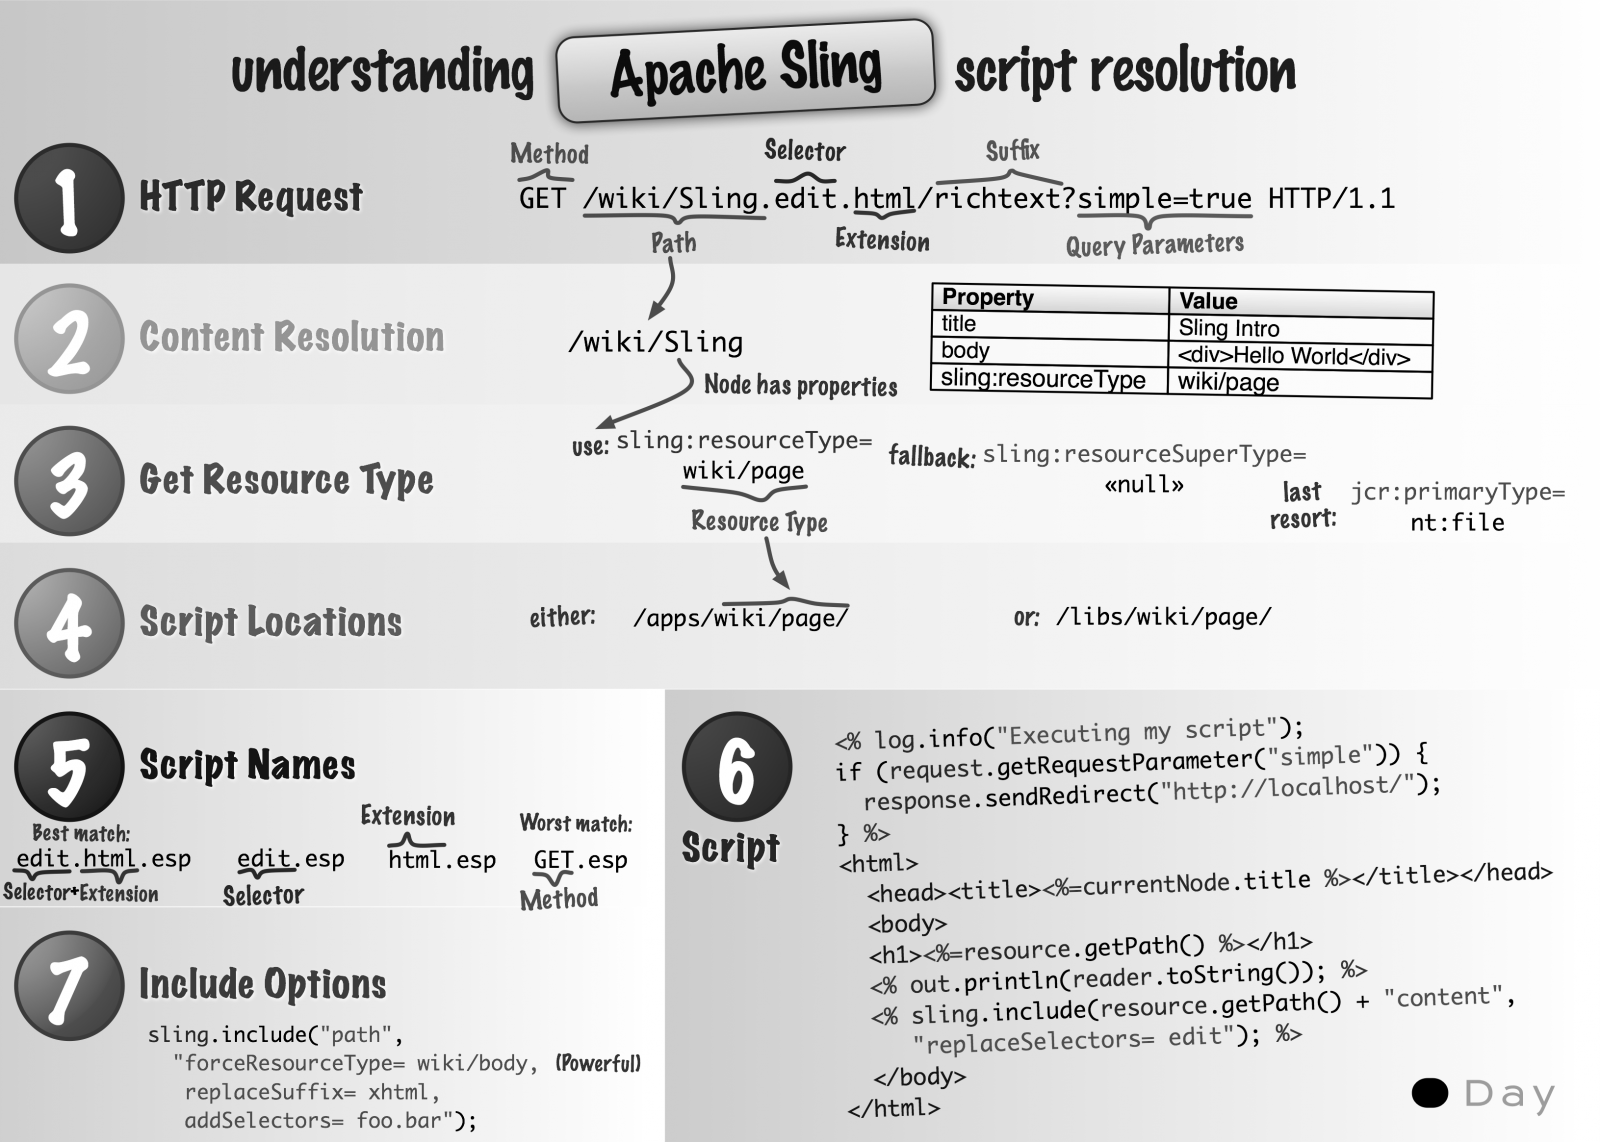
\includegraphics[width=1\textwidth]{sling_bw.png}
		\caption{Auflösung einer Anfrage bei unter Sling, von \cite{adobe_sling}}
		\label{img:sling}
	\end{center}
\end{figure}

Wird z. B. die Seite über einen Webbrowser \pseudourl{http://localhost:4502/wiki/Sling.edit.html/richtext?simple=true} aufgerufen, so wird die URL aufgeteilt. Alles ab \quotes{/wiki...} wird von Sling aufgelöst, somit wird im Folgenden nur der Abschnitt ab \quotes{/wiki...} betrachtet.
\begin{enumerate}
	\item Alles bis zum ersten Punkt ist der Pfad, gefolgt von einem oder mehreren Selektoren und zuletzt der Erweiterung. Anschließend können noch Suffixe und Parameter folgen, die noch weitere Informationen mitgeben.
	\item Die Eigenschaften des Knotens, die sich aus dem vorherigen Schritt erschlossen haben, werden abgefragt und nach einer mit dem Namen. \quotes{sling:resourceType} gesucht. Diese hat in diesem Beispiel den Wert \quotes{wiki/page}.
	\item Der Wert wird für den nächsten Schritt verwendet.
	\item Nun wird zunächst unter /app/wiki/page nach einem geeigneten Skript gesucht. Wird dieses nicht gefunden, wird die Suche unter /libs/wiki/page fortgesetzt.
	\item Der Name des gesuchten Skripts wird aus dem Selektor und der Erweiterung zusammengesetzt. Sollte kein entsprechendes Skript gefunden werden, wird zuletzt noch als Name die Methode ausprobiert.
	\item Wird ein entsprechendes Skript gefunden, kann dieses gerendert werden, und es können z. B. die Parameter, die mit der URL mitgegeben wurden, einfügt werden.
	\item \missing{???}
\end{enumerate}

\paragraph{Autoren-Bedienoberfläche}
\label{sec:autor_ui}\index{Autoren-Bedienoberfläche}
\ac{aem} ermöglicht es Autoren, ihre Webinhalte über zwei Bedienoberflächen zu gestalten. Dies wäre zum einen die klassische Oberfläche, welche für Desktop-PCs ausgelegt ist, und zum anderen die Touch-optimierte für Tablets und Smartphones. Jeder Autor kann sich eine Oberfläche nach Belieben aussuchen und ggf. nachträglich zur jeweils anderen wechseln.\\
Da die Touch-optimierte Bedienoberfläche nach der Installation von \ac{aem} als Standard eingestellt ist und auch auf dem Desktop-PC lauffähig ist, werden sich die folgenden Kapitel, sofern nicht anders erwähnt, mit dieser Oberfläche befassen. \\
Die Autoren-Bedienoberfläche bietet zahlreiche Werkzeuge, um Webseiten nach Belieben zu gestalten. Dazu gehört der Bearbeitungsmodus für Seiten, zu sehen in \autoref{img:aemui}.

\begin{figure}[H]
	\begin{center}
      	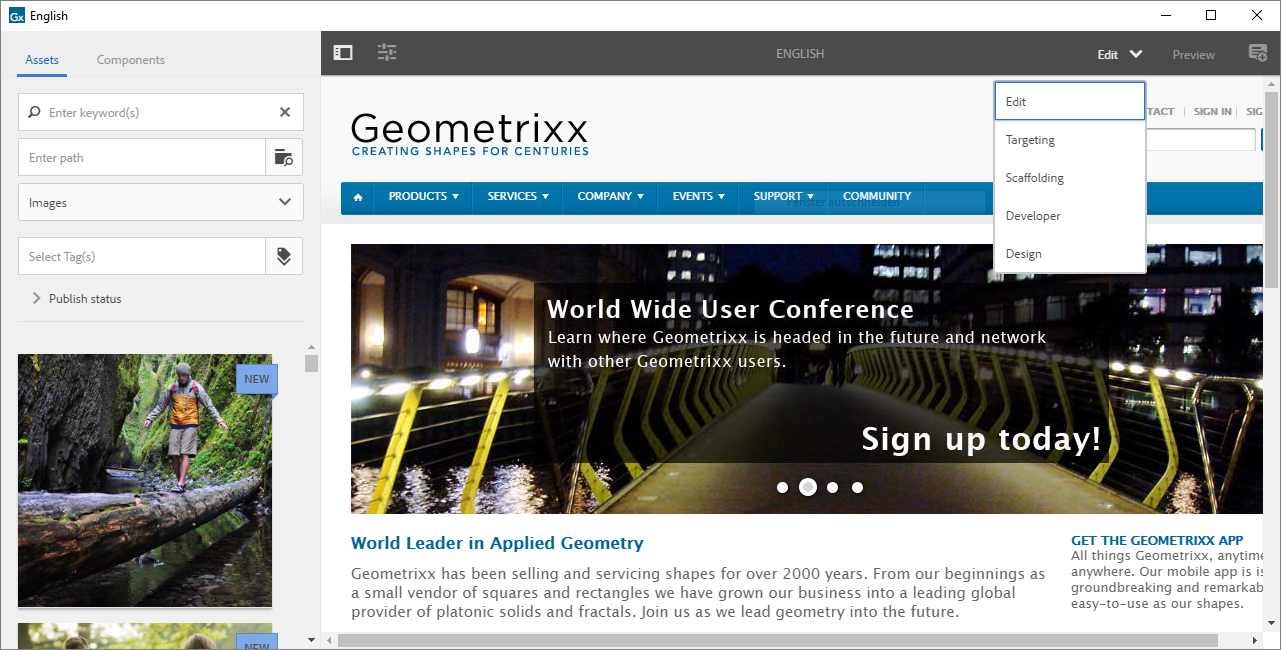
\includegraphics[width=1\textwidth]{aem_autoren_ui.png}
		\caption{Autoren-Bedienoberfläche}
		\label{img:aemui}
	\end{center}
\end{figure}

Das linke Menü lässt sich nach Bedarf auf- und zuklappen. Unterschreitet das Browserfenster eine gewisse Breite, nimmt das Menü dessen gesamte Fläche ein. Hier können Inhalte (Bilder, Dokumente etc. ) und Komponenten durch Ziehen und Loslassen der Seite hinzugefügt werden. In der oberen rechten Ecke wird zwischen verschiedenen Modi gewechselt. Diese sind:

\begin{description}
	\item[Edit:] Inhalte, Texte und Komponenten können eingefügt, entfernt und bearbeitet werden.
	\item[Targeting:] Verwendung des Zusatzproduktes Adobe Target, Teil von \ac{amc}.
	\item[Scaffolding:] Zum Erstellen von mehreren Seiten mit ähnlichem Aufbau.
	\item[Developer:] Für Entwickler, um Komponenten zu debuggen.
	\item[Design:] Hier wird das Design der Seite angepasst.
\end{description}

\paragraph{Administrator Bedienoberfläche}
\ac{aem} bietet einige Werkzeuge an, mit deren Hilfe das System administriert und erweitert werden kann. Zum Beispiel wäre hier eine Bedienoberfläche für die OSGi-Verwaltung und für administrative Eingriffe in das \ac{crx} zu nennen.\\
Entwickler müssen häufig Eigenschaften und Knoten des \ac{crx} editieren. Eine Möglichkeit, dies zu bewerkstelligen, wäre mit dem Tool CRXDE Lite, welches ebenfalls über den Webbrowser erreichbar ist, und es wird bei \ac{aem} per Standard mit installiert. \\
\autoref{img:crxde} zeigt einen Beispielknoten innerhalb einer lauffähigen \ac{aem}-Webanwendung, welche für Lernzwecke mit dem \ac{aem} installiert werden kann.

\begin{figure}[H]
	\begin{center}
		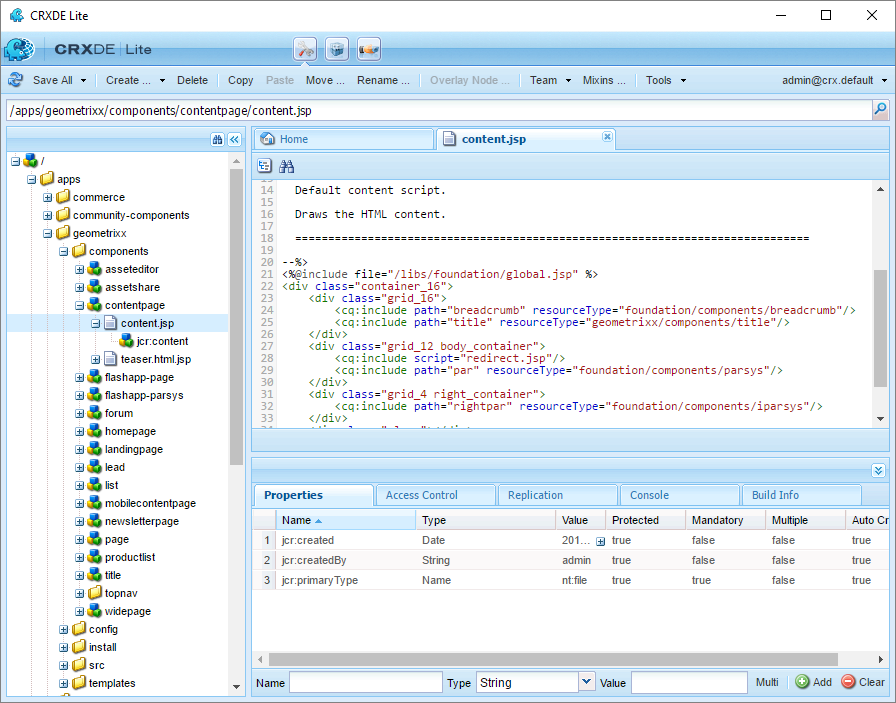
\includegraphics[width=1\textwidth]{crxde.png}
		\caption{CRXDE Lite}
		\label{img:crxde}
	\end{center}
\end{figure}

Wie sich der Abbildung entnehmen lässt, wird die Baumstruktur auf der linken Seite angezeigt. Unten rechts sind die Eigenschaften des gewählten Knotens zu sehen und oben rechts lassen sich Templates und Java-Dateien bearbeiten.
\paragraph{AEM-Anwendung}
\index{AEM Anwendung}
In AEM basieren Webpräsenzen auf AEM-Anwendungen. Dies sind Strukturen im \ac{jcr} und sie befinden sich in der Regel unter \hl{/app} \cite[S. 6.4]{Incorporated2015}. \\
Die übliche Struktur einer Anwendung mit dem Namen helloworld ist in \autoref{lst:aem-anwendung} zu sehen.

\begin{lstlisting}[style=jcr,caption=Exemplarische Darstellung einer AEM Anwendung, label=lst:aem-anwendung]
/apps/helloworld
  + components
  + templates
  
\end{lstlisting}

Unter \hl{/apps/components} werden für die Anwendung spezifische Komponenten, siehe \autoref{sec:komponenten}, abgelegt. Unter Templates befinden sich JSP- und HTL- Vorlagen für die einzelnen Seiten.
\paragraph{HTL}
\label{sec:htl}\index{HTL}
Auch AEM verwendet Templates für seine Seiten. Als Model dienen Daten, welche über die \ac{jcr}-\ac{api} gewonnen werden. Als Template-Sprache kann man zwischen jener von \ac{jsp}\index{JSP} oder auch \ac{htl} wählen. Letztere wurde von Adobe entwickelt und in \ac{aem} mit der Version 6.0 ausgeliefert und wird von Adobe als bevorzugte Templatesprache genannt \cite{Adobe2016}. \\
\ac{htl} ist an \ac{html} angelehnt, somit ist auch jedes in \ac{htl} verfasste Template zugleich gültiges HTML5 \cite[S. 5.11 f.]{Incorporated2015}. Mit dem folgenden \autoref{lst:htl} würden vom aktuellen \ac{jcr}-Knoten alle Kinder in einer HTML-Liste dargestellt und jeder Listeneintrag abwechselnd mit der HTML-Klasse \quotes{odd} bzw. \quotes{even} versehen werden.


\begin{lstlisting}[style=htmlcssjs, caption=Ein HTL Beispiel, label=lst:htl]
<ul data-sly-list.child="${currentPage.listChildren}">
	<li class="${ childList.odd ? 'odd' : 'even'}">${child.title}</li>
</ul>
\end{lstlisting}
\paragraph{Komponenten}
\label{sec:komponenten}
Komponenten in \ac{aem} sind wiederverwendbare modulare Zusammenschlüsse von spezifischen Funktionalitäten, die zur Darstellung von Inhalten auf einer Webpräsenz dienen \cite{Adobe2016a}. \\
Diese werden über die Autoren-Bedienoberfläche an ihren bevorzugten Ort innerhalb einer Webseite platziert, konfiguriert und ggf. wieder gelöscht. \\
AEM liefert bereits einige vorgefertigte Komponenten mit, wie eine Text-Komponente zum Bearbeiten von Text, eine Bild-Komponente, mit der Bilder platziert werden können, und einige mehr. Diese sind in JSP oder HTL geschrieben worden und wurden für die Touch-optimierte, klassische oder für beide Bedienoberflächen entworfen. Hier beschriebene Komponenten sind immer in \ac{htl} geschrieben und für die Touch-optimierte Bedienoberfläche ausgelegt. Die Logik der Komponenten kann in Java, JavaScript und mit Clientlibs erfolgen.
\paragraph{Clientlib}
\label{sec:clientlib}\index{Clientlib}
JavaScript und CSS können durch sogenannte Client Libraries oder kurz auch Clientlib ausgeliefert werden. Dies sind einfache Knoten mit einer bestimmten Struktur und Eigenschaften, welche sich in der Regel innerhalb einer Komponente oder unter \filefolder{/etc/cliebtlibs} befinden. \autoref{lst:clientlib} zeigt exemplarisch die benötigte Struktur und ihre Eigenschaften.

\begin{lstlisting}[style=jcr, caption=Exemplarische Darstellung einer Clientlib, label=lst:clientlib]
/etc/clientlibs/angularapp
  - jcr:primaryType (Name) = cq:ClientLibraryFolder  # Indiziert Knoten als Clientlib
  - categories (String[]) = [angularApplication]     # Ein Array an Kategorien, an dem die Clientlib idendifiziert wird.
  - dependencies (String[]) = [angularjs]            # Mögliche Abhängigkeiten zu anderen Clientlibs
  - embedded (String[]) = [app1, app2]               # Andere Clientlibs können hier eingebettet werden
  + js.txt                                           # Auflistung aller JavaScript Dateien
    - jcr:primaryType = nt:file
  + css.txt                                          # Auflistung aller CSS Dateien
    - jcr:primaryType = nt:file
  + scripts                                          # Ordner für Scripte
    - jcr:primaryType (Name) = nt:folder
  + styles                                           # Ordner für CSS
    - jcr:primaryType (Name) = nt:folder
\end{lstlisting}

Die Ordnernamen für CSS und JavaScript sind hierbei frei wählbar und können auch Unterordner beinhalten. Auch eine Platzierung direkt unterhalb des clientlib-Knotens ist möglich.\\
Innerhalb eines Templates wird nun die Clientlib mithilfe eines entsprechenden Tags verwendet. Dieser würde bei \ac{htl} wie in \autoref{lst:clientlib} aussehen.

\begin{lstlisting}[style=htmlcssjs,caption=Verwendung einer Clientlib in AEM, label=lst:clientlib_useage]
<sly data-sly-use.clientlib="/libs/granite/sightly/templates/clientlib.html" data-sly-unwrap/>
<sly data-sly-call="${clientlib.all @ categories='angularApplication'}" data-sly-unwrap/>
\end{lstlisting}

Zeile 1 wird für den Einsatz von Clientlibs benötigt. Zeile 2 gibt an, welche Clientlib verwendet werden soll. Durch clientlib.all werden alle Ressourcen der Clientlib geladen, clientlib.js und clientlib.css würde nur das Laden der JavaScript- bzw. CSS-Dateien bewerkstelligen. Der Wert hinter categories gibt ein Array an Kategorien an. Nun werden alle Clientlibs samt ihren Abhängigkeiten, welche diesen Kategorien entsprechen, geladen.




